\section{Responsive Design}
Mobile phones and handheld devices are reshaping how we view technology. Their portable nature and accessibility have meant that a growing number of the worlds popultion own a mobile phone. In 2017, a predicted 4.77 billion people worldwide own a mobile phone \cite{Statista:Mobile}, more than half of the global population. An even more staggering statistic is that roughly half of the mobile phones owned are smartphones \cite{Statista:Smartphones}. Smartphones have broadened the scope of internet availability through the advanced capabilities most modern smartphones come equipped with. In fact, for the first time ever in 2016, internet traffic from mobile phones and tablets exceeded that of desktops, accounting for 51.3\% of internet usage \cite{StatCounter:MobileInternetTraffic}. Taking all of this into consideration, it would make no sense to design a web application only fit for purpose on desktops; there must be thought put into building a web application suitable for any and all devices. To this end, Fidelis must guarantee usability regardless of the device it is accessed from, as long as a modern browser is used. For smaller devices, navigation will be hidden to make more room for content on the page. In addition to this, content will be resized based on the size of the screen so that it is clearer and can be read easily without having to pan in and out.

\begin{figure}[H]
	\centering
	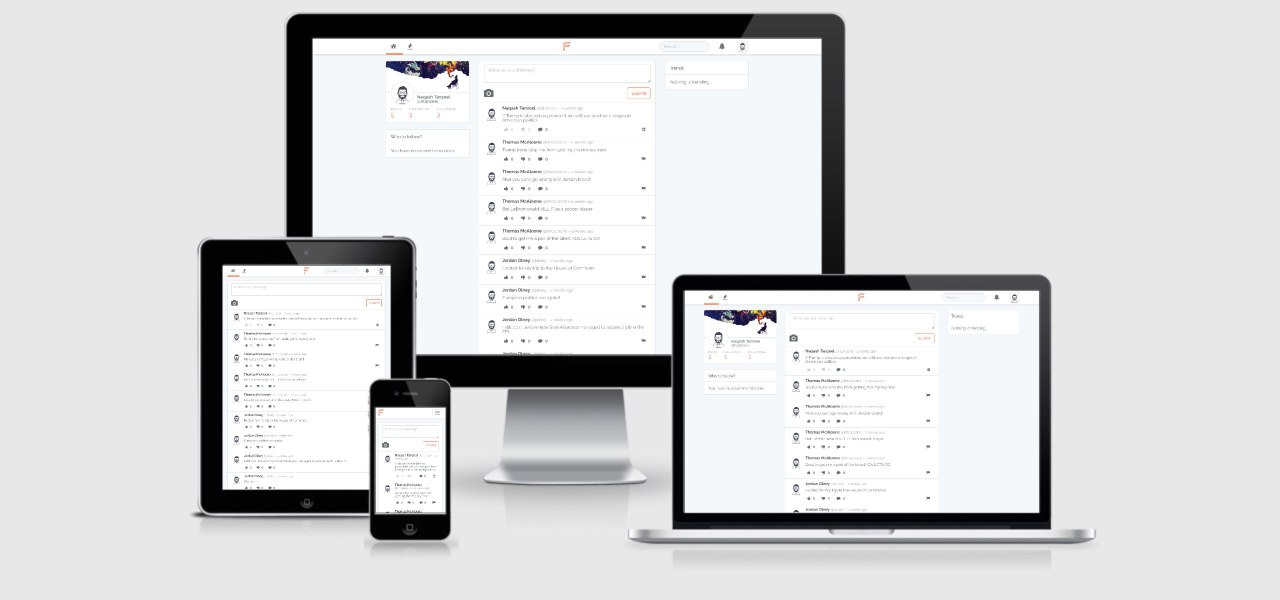
\includegraphics[height=2.5in]{Images/Design/ResponsivePages}
	\caption{Fidelis home page conceptualised across a number of devices}
	\label{fig:responsive}
\end{figure}

Consideration of mobile and handheld devices will strongly influence the design decisions made as certain features will be achievable on devices with lower resolutions whereas other features will make pages appear empty on larger resolution devices. Figure \ref{fig:responsive} shows the profile page as it will appear on devices of varying sizes. In both designs, we see some features are hidden. For example, on the mobile device, the navigation bar is condensed into a menu button which the user can touch to reveal the same options available normally. 